\subsection{The brick experiment}\label{sec:brick}
An instantaneous version of the brick benchmark is performed to verify the correctness of the pressure-dependent plasticity for different angle of internal
friction, as proposed by \citet{Glerum2018}. The domain is rectangular with $L_x=$ \SI{40}{\km} and $L_y=$ \SI{10}{\km} and a grid resolution of $512\times128$
elements. The gravity acceleration is set to $g_y=$ \SI{-10}{\m\square\s} and effective viscosity is capped using $\eta_{min}=$ \SI{e19}{\pascal\s} and
$\eta_{max}=$ \SI{e26}{\pascal\s}. The tolerance for the convergence of the non-linear solution is $tol=10^{-7}$, with a maximum number of non-linear iterations
set to 1000. A 800 m-wide and 400 m-height inclusion with $\eta_b=$ \SI{e20}{\pascal\s} and $\rho_b=$ \SI{2700}{\kg\per\cubic\m} is placed at the bottom of the
domain at $x=L_x/2$. The inclusion is surrounded by a non-linear viscous medium with $\rho_m=$ \SI{2700}{\kg\per\cubic\m}, an initial viscosity of
\SI{e23}{\pascal\s}, a linear viscous viscosity of \SI{e25}{\pascal\s} and a cohesion of \SI{40}{\mega\pascal}. Velocities are set to free slip conditions at
the bottom of the domain and the top is open. Velocities on sides of the domain are fixed to $u=$ \SI{+-2e-11}{\m\per\s} and $v=0$. The experiment is performed
in compressional and extensional contexts with an angle of internal friction $\phi$ of the non-linear medium variable between 0° and 30°.

As expected, two shear bands stem from the inclusion with variable angles in relation to both the dynamics context and the internal friction angle. Shear band
angles formed at 45° for $\phi=0$° in both extensional and compressional contexts (Fig. \ref{fig:brick_beam}a), while they are different in case of $\phi\neq0$°.

\begin{wrapfigure}{r}{12.5cm}
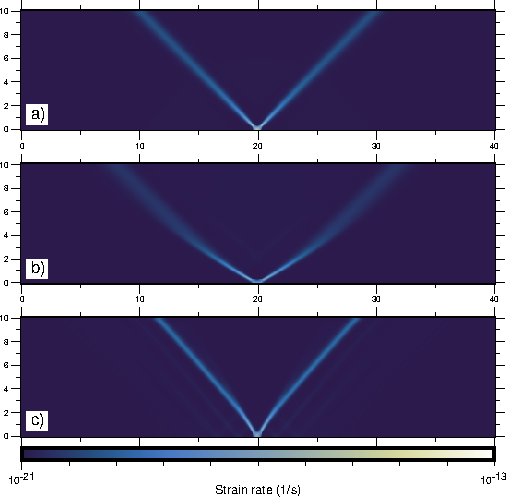
\includegraphics[width=12.5cm]{./Figures/Brick_Beam.pdf}
\caption{Shear band angles predicted for the brick experiment for $\phi=0$° (panel a) and for $\phi=20$° in case of compression and extension (panels b and c,
respectively).}
\label{fig:brick_beam}
\end{wrapfigure}
Shear band angles in case of $\phi=20$° are shown for compression and extension in Fig. \ref{fig:brick_beam}b  and c, respectively.
Values of shear band angles as function of internal friction angles from 0° to 30° are extracted at different depths and minimum and maximum values are plotted in Fig. \ref{fig:brick},
in comparison with theoretical Roscoe, Arthur and Coulomb shear band angles. For all tests the tolerance for nonlinear convergence is defined $tol=10^{-7}$
and none converges before the maximum number of iterations ($it_{max}=1000$) is reached. However, tests with internal friction angles up to 15° show a constant
decrease of the velocity residuals, which can not be observed for for tests with higher internal friction angles (Fig. \ref{fig:convergence}). 
All data can be found at \url{https://github.com/aleregorda/Benchmarks/tree/main/Nonlinear_visco_plasticity/Brick_experiment}.

\begin{figure}[h]
\centering
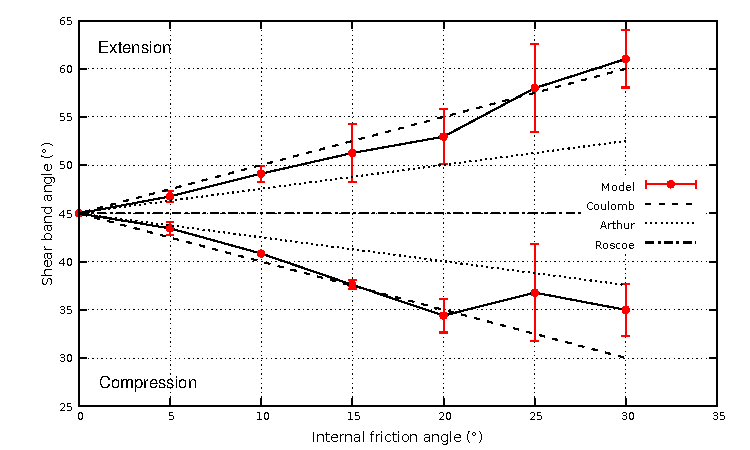
\includegraphics[width=12cm]{./Figures/Brick.pdf}
\caption{Shear band angles predicted for the brick experiment in case of compressional and extensional contexts as function of different internal angle of
friction (continuous black line and red dots), compared with theoretical Roscoe, Artur and Coulomb angles (discontinuous black lines). Red lines indicate the
range of angles calculated at different depths.}
\label{fig:brick}
\end{figure}

\begin{figure}[h!]
  \centering
  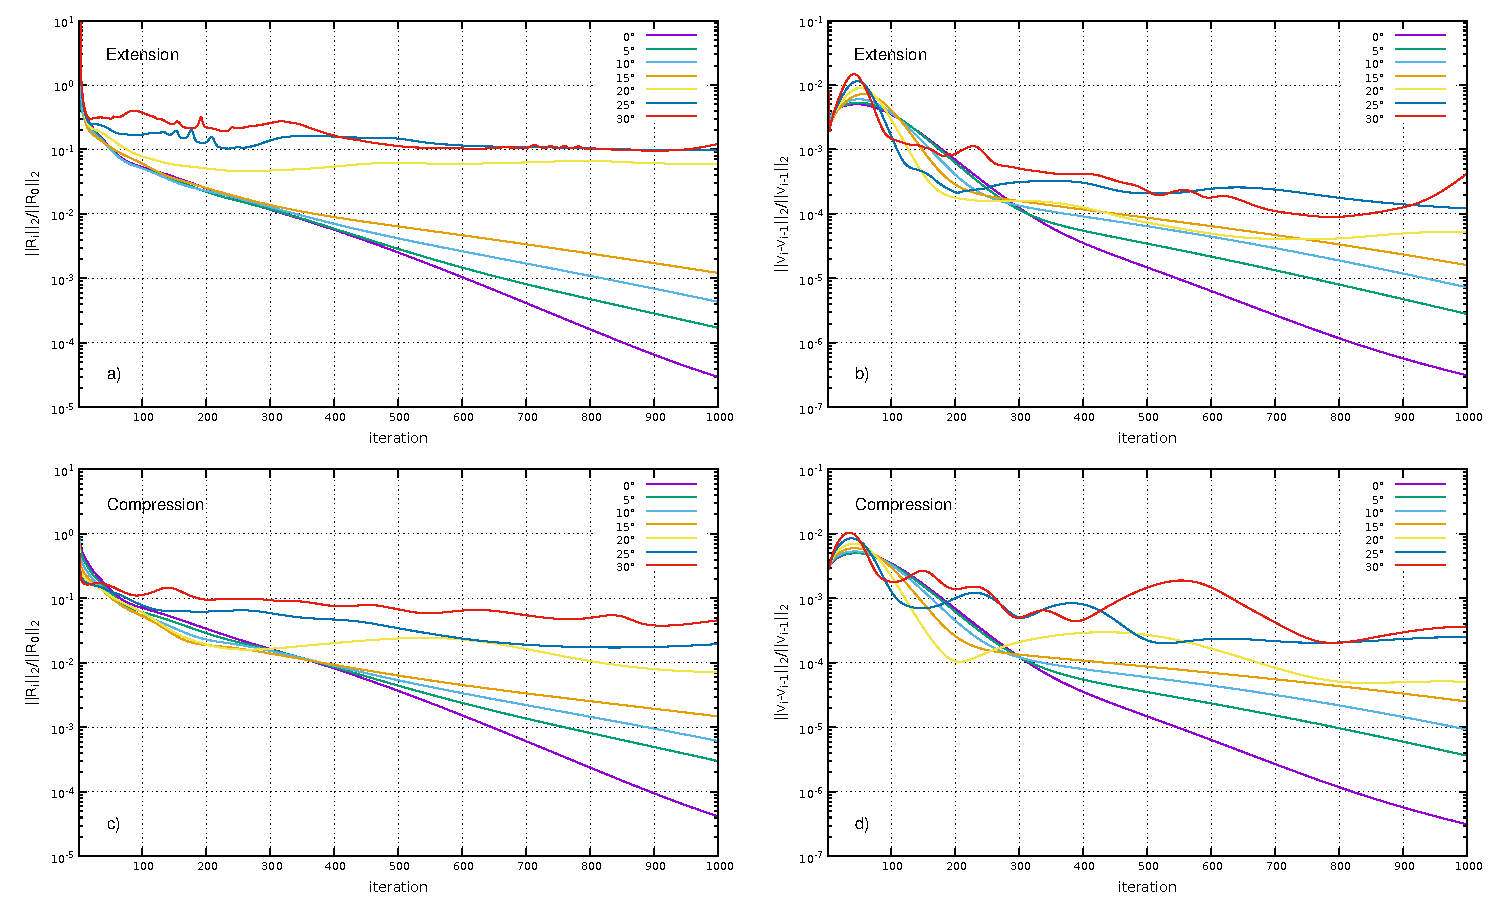
\includegraphics[width=15cm]{./Figures/convergence.pdf}
  \caption{Convergence rates for all tests. Normalised residuals (left column) are compared with velocity residuals (right column) for extensional (first row)
  and compressional (second row) settings.}
  \label{fig:convergence}
  \end{figure}